\documentclass{standalone}
\usepackage{tikz}

\begin{document}

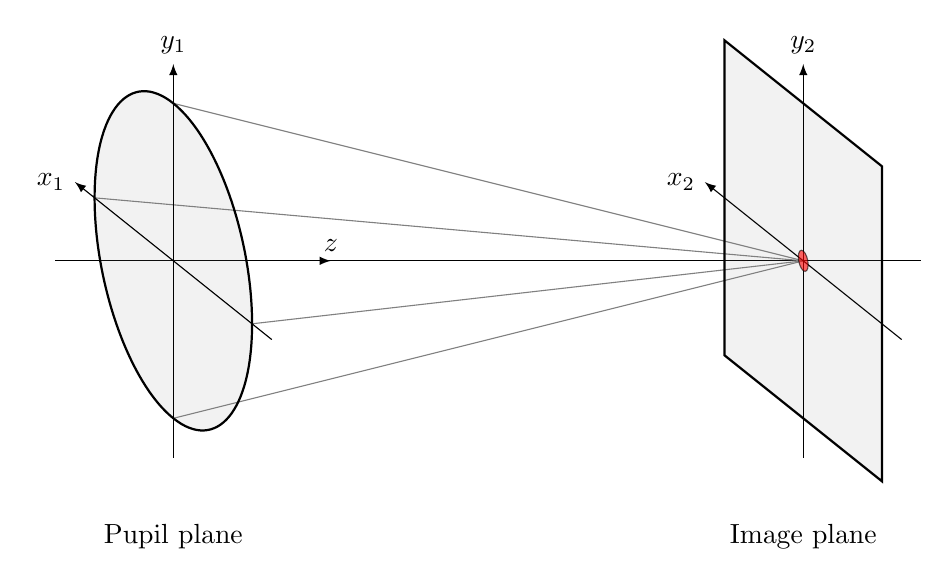
\begin{tikzpicture}[z={(1cm,0cm)},x={(0.5cm,-0.4cm)}, y={(0cm,1cm)}, scale=1]

    % constants
    \def\zimg{8}

    % coordinate system
    \coordinate (0) at (0,0,0);
    \coordinate (2) at (0,0,\zimg);

    % optical axis
    \draw[-latex] (0) -- +(0,0,2) node [above] {$z$};
    \draw (0,0,-1.5) -- (0,0,9.5);


    % Aperture plane
    \draw[color=gray] (-2,0,0) -- (0,0,\zimg);
    \draw[color=gray] (2,0,0) -- (0,0,\zimg);
    \draw[color=gray] (0,-2,0) -- (0,0,\zimg);
    \draw[color=gray] (0,2,0) -- (0,0,\zimg);

    \draw[thick, fill=gray, fill opacity=0.1] (0,0) circle [radius=2];
    \draw[latex-] (-2.5,0,0) node [left] {$x_1$} -- (2.5,0,0);
    \draw[-latex] (0,-2.5,0) -- (0,2.5,0) node [above] {$y_1$};


    \node [align=left] at (0,-3.5,0) {Pupil plane};

    % Observation plane
    \draw [thick,fill=gray,fill opacity=0.1] (-2,-2,\zimg) -- (2,-2,\zimg) -- (2,2,\zimg) -- (-2,2,\zimg) -- cycle;
    \draw[latex-] (-2.5,0,\zimg) node [left] {$x_2$} -- (2.5,0,\zimg);
    \draw[-latex] (0,-2.5,\zimg) -- (0,2.5,\zimg) node [above] {$y_2$};

    \node [align=center] at (0,-3.5,\zimg) {Image plane};

    % psf location
    \draw[fill=red, opacity=0.6] (0,0,\zimg) circle [radius=0.125];

\end{tikzpicture}

\end{document}
